%\newcommand{\sys}{Combo}

\section{Model Decomposition and Synthesis (MDS)}
%描述过程和具体设计(软件工程详细设计
\subsection{Worker Proactive Pulling}
When a node $i$ finishes the local training and seeking to do the model aggregation, it reports its status to the index server. And then the server randomly samples a subset $K_i$ from all the participating nodes as the aggregation candidates of node $i$ and send the information about $K_i$ to node $i$. To control the training progress, the nodes of $K_i$ should have the same training iterations. When node $i$ receives the candidate list $K_i$, it proactively fetches the model from the candidate nodes, do the aggregation and then continue training on the local dataset. We use an index server to track the information of nodes instead of storing peer information on the nodes directly because with the growth of the nodes and the variation of the network environment, the synchronization overhead can be very huge.

 By increasing the initiative of the nodes, the bottleneck of server is removed because the communication of the server is trivial and the model parameters, which is the heavy part, are transferred among $n(n-1)$ links of all the nodes.

\subsection{Worker Segmented Transfer and Aggregation}
After ... , the worker will ... transfer and aggregation...
% 一句话描述他们要干什么
\sys borrows the idea of ...

The idea of pulling model parameters from peers is quite similar with the Gossip-based protocols in which the nodes randomly push the models to others. So they are facing the same challenge that the overall transmission quantity is increased for a single node. In the traditional parameter server architecture, in one global iteration, the node only has to send and receive for one time. But with the gossip methods, each node is expected to send and receive for $|K_i|$ times in one iteration. 
\subsubsection{Segmented Transfer}
% 描述详细的设计
Let $\mathcal{W}$ denote the model parameters, we break $\mathcal{W}$ into $S$ segments such that:
\begin{equation}
    \begin{split}
        \bigcup_{l = 1}^{S} \mathcal{W}[l] &= \mathcal{W} \\
        \mathcal{W}[l] \cap  \mathcal{W}[m] &= \emptyset \quad \forall l\neq m
    \end{split}
\end{equation}
The segment process doesn't have to be sequential as long as it follows the above requirement, but the segment rule must be clear, that is for any model parameter, you have to know which segment it belongs to. 

When the node $i$ receives the candidate list $K_i$ from index server. For each segment $l$, node $i$ randomly choose a node $N_l$ from the candidate list, and then fetch the corresponding segment from node $N_l$ which we denote as $\mathcal{W}[l;N_l]$. Note that this step can be parallelized. When it fetches all the segments back, a new mixed model can be rebuilt as:
\begin{equation}
    \mathcal{W}^\prime = \bigcup_{l = 1}^{S} \mathcal{W}[l;N_l] \label{eq:seg_union}
\end{equation}

With the segmented transfer method, node $i$ receives model information from multiple peers with the transfer size equal to one model. Thus in the aggregation phase, the aggregation result can be affected by more datasets and this could help to increase the generality of the model. But if the number of the participating nodes is too big, which could be common in a federated learning context, the segments can only cover few nodes. Increasing the number of segments might help but an extremely small segment size could lead to over-mottled parameters. Thus as a compromise, we set a hyper-parameter $R(eplica)$ which means the number of the mixed model rebuilt by Segmented Transfer. 

Another shining point of segmented transfer is privacy preserving. The complete model parameter or gradient set has the potential to leak private data information under attack. Instead of pulling the whole model from peers, \sys only collects a random subset of the parameters, which helps to preserve the data privacy. 


 \begin{figure}[H]
\centering 
\subfigure[Segment Transfer]{
\label{Fig: Segment sub.1}
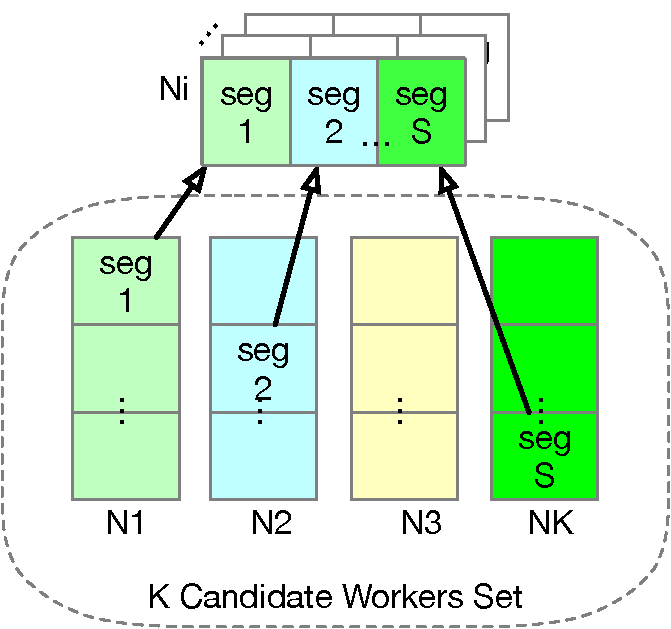
\includegraphics[width=0.225\textwidth]{pics/transfer.pdf}}
\subfigure[Segment Aggregation]{
\label{Fig.Segment sub.2}
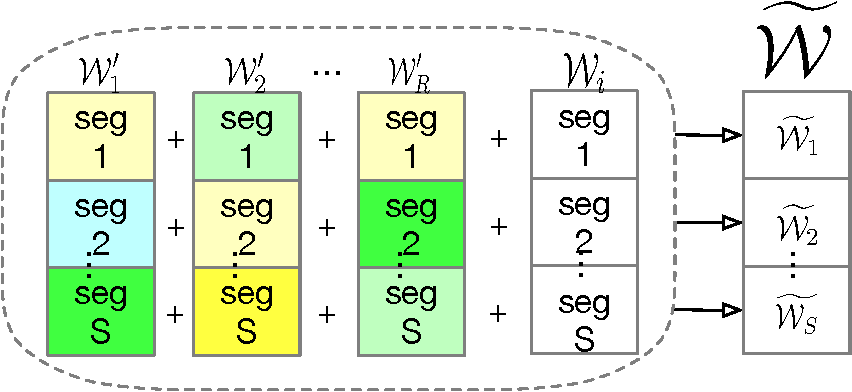
\includegraphics[width=0.225\textwidth]{pics/aggregation.pdf}}
\caption{Segment Transfer and }
\label{Fig: Segment}
\end{figure}

\subsubsection{Segmented Aggregation}
Typically the model aggregation uses weighted mean of the model parameters with the node's dataset size as weight. But in \sys, the mixed models are patched together so it is hard to set a reasonable weight for the mixed model as a whole. For such case, we use a segment-wise model aggregation in \sys.

 Assume the node $i$ has has fetched all the segments and rebuilt $R$ mixed models which we represent as $\mathcal{W}^\prime_1,\mathcal{W}^\prime_2, \dots ,\mathcal{W}^\prime_R$. Let $\mathcal{W}$ denote the model parameters of node $i$. First, we break $\mathcal{W}$ to $S$ segments using the same rule as the segmented transfer. Then for each segment $l$, we have $R$ mixed models and 1 local model to aggregate. Let $P_l$ denote the set of the nodes which provide the segment $l$(node $i$ is contained too) and $|D_j|$ denote the dataset size of node $j$, then we can aggregate segments $l$ by:
 \begin{equation}
     \widetilde{\mathcal{W}}[l] = \frac{\sum_{j\in P_l}|D_j|\mathcal{W}[l;j]}{\sum_{j\in P_l}|D_j|}
 \end{equation}

With all the aggregated segments $\widetilde{\mathcal{W}}[l]$, we can rebuild the final result by using \eqref{eq:seg_union}. And then the node can continue its training until next aggregation phase comes.

\subsection{Server Dynamic Configuration}

\subsubsection{Available Worker Updates}


\subsubsection{Fault Tolerence}
In the context of federated learning, the participating nodes are more likely to be mobile phones and embedded devices, which are often not connected to a power supply and stable network. To ensure the availability of the devices, traditional distributed systems adopt the heartbeat packet and time threshold to determine the status of the nodes. However, these methods are not applicable with federated learning for next two reasons: 1) The server has to maintain the heartbeat connection with all the participating nodes which limits the scalability of the system. 2) The computation times of each nodes vary greatly due to the difference of the computing devices and network environment.

Fortunately, the design of \sys gives us an opportunity to solve this problem decently. In the normal situation, when a node comes to the federation, it just has to register itself on the index server, pull the newest model segments to rebuild a model as its own, and then it's in. When it quits, it should wipe out its record at index server so other nodes won't request its model.

And the interesting thing is that when the node exits accidentally, it doesn't affect the federation at all. The node won't be noticed if no one requests model from this node. And if a node does randomly chooses this absent node as its target and fails to connect, it just has to select another node and report the absence to the server. Then the server know it's time to stop providing this absent node as candidate and delete the record. And if it is a false report due to the network connection, the index can be quickly rebuilt as long as the communication between the absent node and the index server reestablished. 